\documentclass[final,hyperref={pdfpagelabels=false},5pt]{beamer}
\usepackage{grffile}
\mode<presentation>{\usetheme{penn}}
\usepackage[english]{babel}
%\usepackage[latin1]{inputenc}
\usepackage{amsmath,amsthm, amssymb, latexsym}
%\usepackage{lmodern}
%\usepackage{times}\usefonttheme{professionalfonts}  % obsolete
%\usefonttheme[onlymath]{serif}
\boldmath
\usepackage[orientation=portrait,size=b1,scale=1.25,debug]{beamerposter}

\usepackage{rigidmath}
\usepackage{mathspec}
%\setmainfont{Times New Roman}
%\setsansfont[Ligatures=TeX, % recommended
   %UprightFont={* Light},
   %ItalicFont={* Light Italic},
   %BoldFont={*},
   %BoldItalicFont={* Italic}]{Open Sans}
%\setmainfont{Garamond Premier Pro}
%\setmathfont{Latin Modern Roman}
%\setmathfont[range=\mathit]{Latin Modern Roman}
%\setmathrm{Latin Modern Roman}
%\usepackage[default,osfigures]{opensans}
%\renewcommand\seriesdefault{l}
%\renewcommand\bfdefault{m}
%\setlength{\paperwidth}{30in}
%\setlength{\paperheight}{40in}
% change list indention level
% \setdefaultleftmargin{3em}{}{}{}{}{}


%\usepackage{snapshot} % will write a .dep file with all dependencies, allows for easy bundling

\usepackage{array,booktabs,tabularx}

\usepackage{tikz}
\usetikzlibrary{arrows}
\usetikzlibrary{arrows.meta}
\usetikzlibrary{patterns,snakes}
\usetikzlibrary{calc}







\newcolumntype{Z}{>{\centering\arraybackslash}X} % centered tabularx columns
%\newcommand{\pphantom}{\textcolor{ta3aluminium}} % phantom introduces a vertical space in p formatted table columns??!!

\DeclareMathOperator*{\argmax}{arg\,max}
\DeclareMathOperator*{\argmin}{arg\,min}

\listfiles

%%%%%%%%%%%%%%%%%%%%%%%%%%%%%%%%%%%%%%%%%%%%%%%%%%%%%%%%%%%%%%%%%%%%%%%%%%%%%%%%%%%%%%
\graphicspath{{figures/}}
 
%\title{\fontspec{Garamond Premier Pro} { Modeling and Analysis of Non-unique Behaviors in Multiple Frictional Impacts }}
%\title{\fontspec{Garamond Premier Pro} {\noindent  \,MODELING AND ANALYSIS OF NON-UNIQUE\, \linebreak \mbox{\,BEHAVIORS} IN MULTIPLE FRICTIONAL IMPACTS\, \linebreak} }
%\title{{\noindent  \,MODELING AND ANALYSIS OF NON-UNIQUE\, \linebreak \mbox{\,BEHAVIORS} IN MULTIPLE FRICTIONAL IMPACTS\, \linebreak} }
\title{{\noindent  \,SAMPLE-EFFICIENT LEARNING OF \, \linebreak \,RIGID BODY DYNAMICS\, \linebreak} }
\author{Samuel Pfrommer (CIS 2021), Mathew Halm (MEAM), Michael Posa (MEAM)}
\institute[University of Pennsylvania]{PURM --- DAIR Laboratory --- University of Pennsylvania}
\date{Feb. 12th, 2018}

%%%%%%%%%%%%%%%%%%%%%%%%%%%%%%%%%%%%%%%%%%%%%%%%%%%%%%%%%%%%%%%%%%%%%%%%%%%%%%%%%%%%%%
\newlength{\columnheight}
\setlength{\columnheight}{31.5in}
%\useinnertheme{rounded}

%%%%%%%%%%%%%%%%%%%%%%%%%%%%%%%%%%%%%%%%%%%%%%%%%%%%%%%%%%%%%%%%%%%%%%%%%%%%%%%%%%%%%%
\begin{document}
\begin{frame}
  \vspace{-26ex}
    \begin{columns}
    % ---------------------------------------------------------%
    % Set up a column 
    \begin{column}{.49\textwidth}
      \begin{beamercolorbox}[center,wd=\textwidth]{postercolumn}
        \begin{minipage}[T]{.95\textwidth}  % tweaks the width, makes a new \textwidth
          \parbox[t][\columnheight]{\textwidth}{ % must be some better way to set the the height, width and textwidth simultaneously
            % Since all columns are the same length, it is all nice and tidy.  You have to get the height empirically
            % ---------------------------------------------------------%
            % fill each column with content  
            \begin{block}{Motivation}
              \color{penndkbl}
                    \begin{itemize}
                        \item Current robots are stuck in repetitive, predictable environments
                        \item Want to enable dynamic interaction with objects
                        \item Frictional contact is fundamental to robot manipulation, but difficult to model
                            \begin{itemize}
                                \item Sudden changes in dynamics when making/breaking contact 
                                \item Stick/slip transitions
                                \item Large regions of zero state gradients w.r.t parameters
                            \end{itemize}
                    \end{itemize}

                \begin{center}
                    \textbf{How can we effectively learn dynamics over a stiff class of models?}
                \end{center}
              \end{block}

              \begin{block}{Model requirements}
                \begin{enumerate}
                    \item True dynamics lies within class of learnable models and is optimal
                    \item Stiffness of underlying model does not directly determine gradients 
                    \item Non-zero gradients exist for a large region of parameter space
                \end{enumerate}
              \end{block}
                      
            \begin{block}{Prior Work}
                \begin{columns}[t]
                    \begin{column}{0.3\textwidth}
                        \textbf{Purely learned}
                        \begin{itemize}
                            \item Often in context of policy learning
                            \item Slow and data innefficient
                            \item Doesn't use existing knowledge of contact dynamics
                        \end{itemize}
                    \end{column}

                    \begin{column}{0.3\textwidth}
                        \textbf{Hybrid}
                        \begin{itemize}
                            \item Best of both worlds
                        \end{itemize}
                        \begin{center}
                            \textit{Approaches:}
                        \end{center}
                        \begin{itemize}
                            \item Sim-to-real
                            \item Residual physics
                            \item \textbf{Differentiation through contact problem}
                        \end{itemize}
                    \end{column}

                    \begin{column}{0.3\textwidth}
                        \textbf{Analytical}
                        \begin{itemize}
                            \item Only an approximation
                            \item Doesn't fully capture real-world phenomena
                        \end{itemize}
                    \end{column}
                \end{columns}
            \end{block}
            

            \begin{block}{Method}
              \begin{enumerate}
                  \item Formulate base contact model as fusion of Drumwright \cite{Drumwrighta} and MuJoCo \cite{Todorov}
                      \textbf{Phase 1:} Solver for normal forces with no friction:
                      \begin{align*}
                          \argmin _{\NormalForce \geq \vect 0} \quad &\NormalForce^T \Jn \Mass^{-1} \Jn ^T \NormalForce + \Jn f \Force \\
                                                            & \Jn \Mass^{-1} \Jn ^T \NormalForce \Delta t + (\Jn f) \Gap \geq 0
                      \end{align*}

                      \textbf{Phase 2:} Compute $\kappa = e^T \NormalForce$ from phase 1. Then solve frictional contact:
                      \begin{align*}
                          \argmin _{\Force} \quad \Force^T \J \Mass^{-1} \J ^T \Force + \J f \NormalForce + & \NormalForce^T diag( exp(\Gap) ) \NormalForce \\
                                               \J \Mass^{-1} \J ^T \Force \Delta t + (\J f) \Gap & \geq 0 \\
                                                                  \NormalForce &\geq 0 \\
                                                                  e^T \NormalForce &\leq \kappa \\
                                                                  \FrictionForce &\leq \mu \NormalForce
                      \end{align*}
                  \item Penalize deviations from measured data in subproblem
                      \begin{itemize}
                          \item Incorporate $L_2$ \textbf{deviation penalty} in contact model objectives
                          \item \textbf{Soften} hard constrants in subproblems
                          \item Introduces a \textbf{tradeoff} between satisfying model and matching experimental observations to avoid nonexistant parameter gradients
                      \end{itemize}
                  \item Optimize model parameter set with respect to summed error over all data points:
                      \begin{align*}
                          \argmin _{\theta} \quad & \sum _i \left(Dynamics(\Configuration _i, \Input _i, \Force) - \bar \Configuration _i \right)^2 \\
                          s.t. \quad &\Force = Sol (\Configuration _i, \Input _i)
                      \end{align*}
                      Where $Sol$ refers to the forces produced by the above subroutine. This outer optimization is performed with gradient descent, where gradients through the QP subproblems are supplied by Amos et. al. \cite{Amos2017}.
              \end{enumerate}
                
              \begin{footnotesize}
                  \begin{center}
              $\Configuration$ -- configuration | $\Input$ -- input | $\NormalForce$ -- normal forces | $\FrictionForce$ -- frictional forces | $\Jn$ -- normal contact Jacobian | $\Jt$ -- tangential contact Jacobian | $\vect f$ -- no contact dynamics | $\Gap$ -- gap function | $\mu$ -- Coulomb friction coefficient | $\Mass$ - inertia matrix
                  \end{center}
              \end{footnotesize}
            \end{block}
            \footnotesize{\color{pennbl}
				\bibliography{library2}
				\bibliographystyle{plain}}
           %\begin{columns}[c]
				%\begin{column}{.25\textwidth}
				
				%\begin{figure}
				
					%
\includegraphics[width=\textwidth]{NSFLogo}
				%\end{figure}
				%\end{column}
				%\begin{column}{.64\textwidth}
				%\centering
				%\begin{figure}
				%\centering
					%
\includegraphics[width=\textwidth]{grasp_logo1_blue}
				%\end{figure}

				%\end{column}
				%\end{columns}
				

    
          }
        \end{minipage}
        
      \end{beamercolorbox}
      
    \end{column}
    %\textcolor{penndkbl}{\vrule}

\hfill
    % ---------------------------------------------------------%
    % end the column

    % ---------------------------------------------------------%
    % Set up a column 
    \begin{column}{.49\textwidth}
      \begin{beamercolorbox}[center,wd=\textwidth]{postercolumn}
        \begin{minipage}[T]{.95\textwidth} % tweaks the width, makes a new \textwidth
          \parbox[t][\columnheight]{\textwidth}{ % must be some better way to set the the height, width and textwidth simultaneously
            % Since all columns are the same length, it is all nice and tidy.  You have to get the height empirically
            % ---------------------------------------------------------%
            % fill each column with content
             \begin{block}{Application: 1d frictional block}
             \begin{columns}[c]
				\begin{column}{.6\hsize}
				\justify
                A simple example of a sliding point-mass with stick-slip friction. If the initial estimate for the friction coefficient $\mu$ is much higher than the actual $\mu$, local changes of $\mu$ will be unable to reward the optimizer (block stays sticking no matter what). Introducing tradeoffs into the subproblem helps create gradients.
				\end{column}
				\begin{column}{.35\hsize}
				\centering
				\vspace{0ex}
    \begin{figure}
            \begin{tikzpicture}
\tikzstyle{ground}=[fill,pattern=north west lines,draw=none,minimum width=5,minimum height=0.7]
\node (wall1) [ground, minimum height=0.6cm, minimum width=5cm] {};
\draw [thick] (wall1.north west) -- (wall1.north east);
\node [draw,minimum width=2cm,minimum height=2cm, thick] (mass) at (0,1.4) {};
\draw [ultra thick, ->] (mass.center) -- +(2.5cm,0cm)  node[right] {$u$};
\draw [ultra thick, ->] (mass.center) -- +(0cm,-3.0cm)  node[right] {$mg$};
\draw [ultra thick, ->] (mass.center) -- +(-1.5cm,0cm)  node[left] {$m g \mu$};
\node [circle, fill=black, inner sep=0cm,minimum size=0.3cm] (b) at (mass) {};
\draw [ultra thick, <->] ($(mass.center)+(-2cm,2cm)$) -- ($(mass.center)+(2cm,2cm)$)  node[right] {$v$};
            \end{tikzpicture}
    \end{figure}
				\end{column}
			 \end{columns}
              \vspace{1ex}
             \begin{center}
             	\textbf{Modification of subproblem produces learnable gradients}
             \end{center}
              \begin{figure}
              	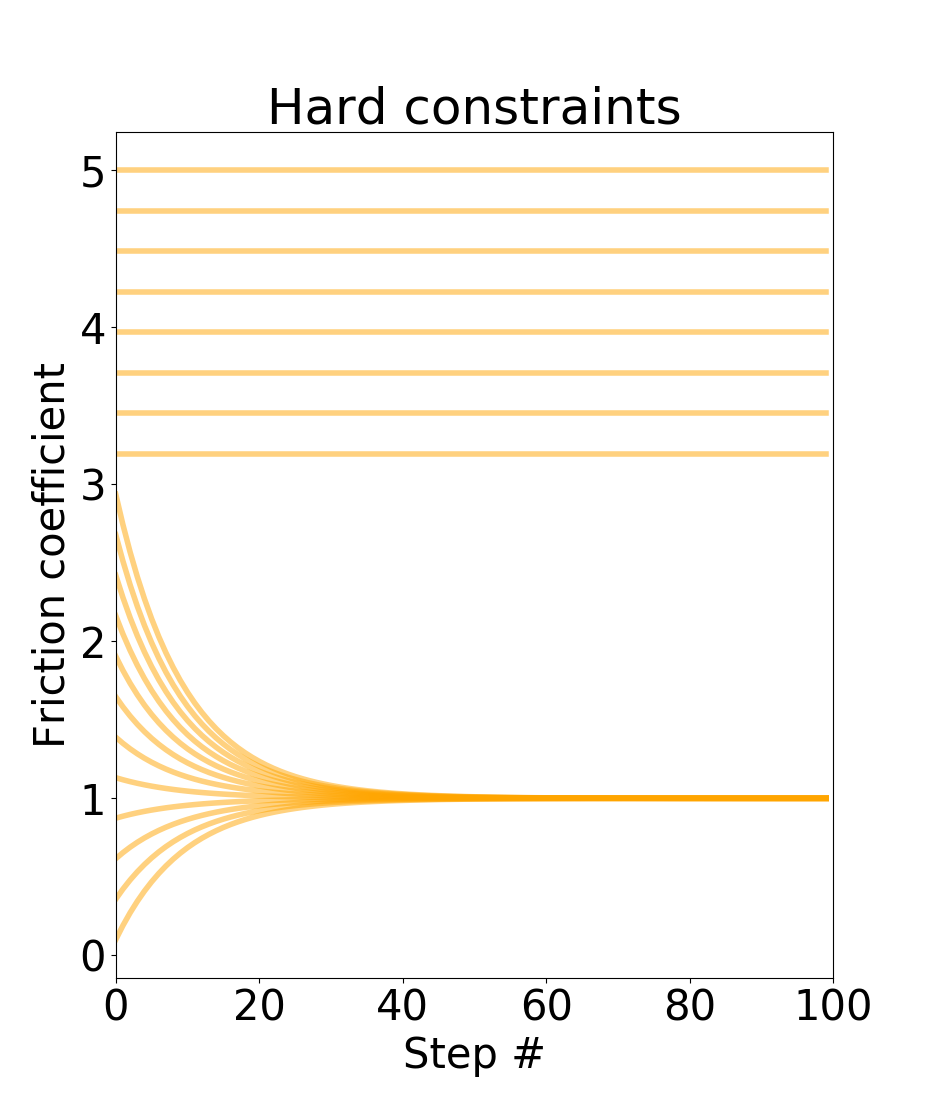
\includegraphics[width=0.4\textwidth]{hard_constraints}
              	\hspace{0.125\textwidth}
              	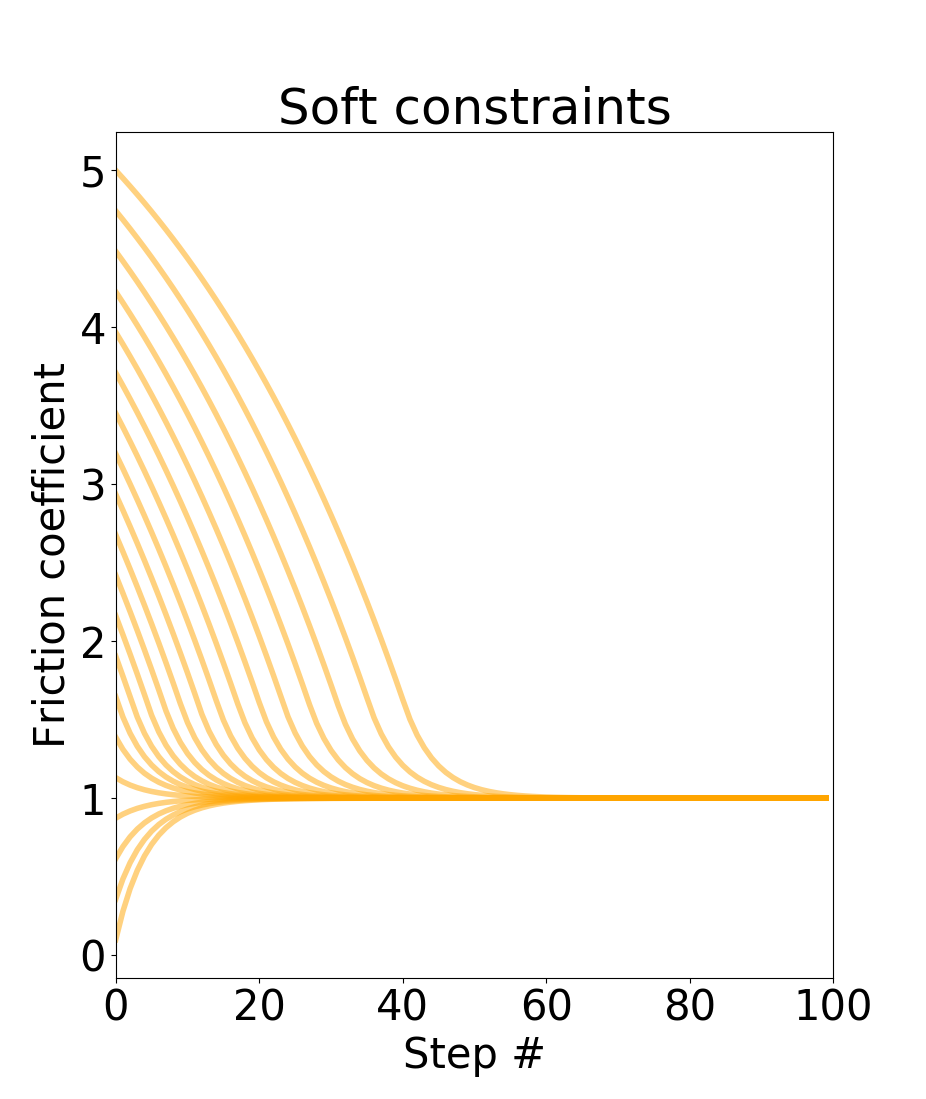
\includegraphics[width=0.4\textwidth]{soft_constraints}
              \end{figure}
            \end{block}
            
             \begin{block}{Application: 2D polygon}
             \centering
             \begin{columns}[c]
				\begin{column}{.6\hsize}
				\justify
                A planar polygon tumbling on a static surface. The forward dynamics can be solved using a variety of different methods; for learning, we used the combined Drumwright / MuJoCo model on the left due to its convenient convex form. Optimization was performed using stochastic gradient descent.
				\end{column}
				\begin{column}{.35\hsize}
				\centering
				\vspace{0ex}
    \begin{figure}
            \begin{tikzpicture}
\tikzstyle{ground}=[fill,pattern=north west lines,draw=none,minimum width=2,minimum height=0.7]
\node (wall1) [ground, minimum height=0.6cm, minimum width=3cm] {};
\draw [thick] (wall1.north west) -- (wall1.north east);
\node [] (mass) at (-0.2,1.6) {};

\coordinate[] (A) at (0,0.4);
\coordinate[] (B) at (1.5,2);
\coordinate[] (C) at (-1,3);
\coordinate[] (D) at (-1.5,0.8);
\draw[thick] (A)--(B)--(C)--(D)--cycle;

\draw [ultra thick, ->] (mass.center) -- +(2.5cm,0cm)  node[right] {$u$};
\draw [ultra thick, ->] (A) -- +(0cm,-3.0cm)  node[right] {$\NormalForce$};
\draw [ultra thick, ->] (A) -- +(-2.5cm,0cm)  node[left] {$\FrictionForce$};
\node [circle, fill=black, inner sep=0cm,minimum size=0.3cm] (b) at (mass) {};
            \end{tikzpicture}
    \end{figure}
				\end{column}
				\end{columns}
              \vspace{1ex}
             \begin{center}
             	\textbf{Simultaneous optimization of multiple parameters}
             \end{center}
              \begin{figure}
              	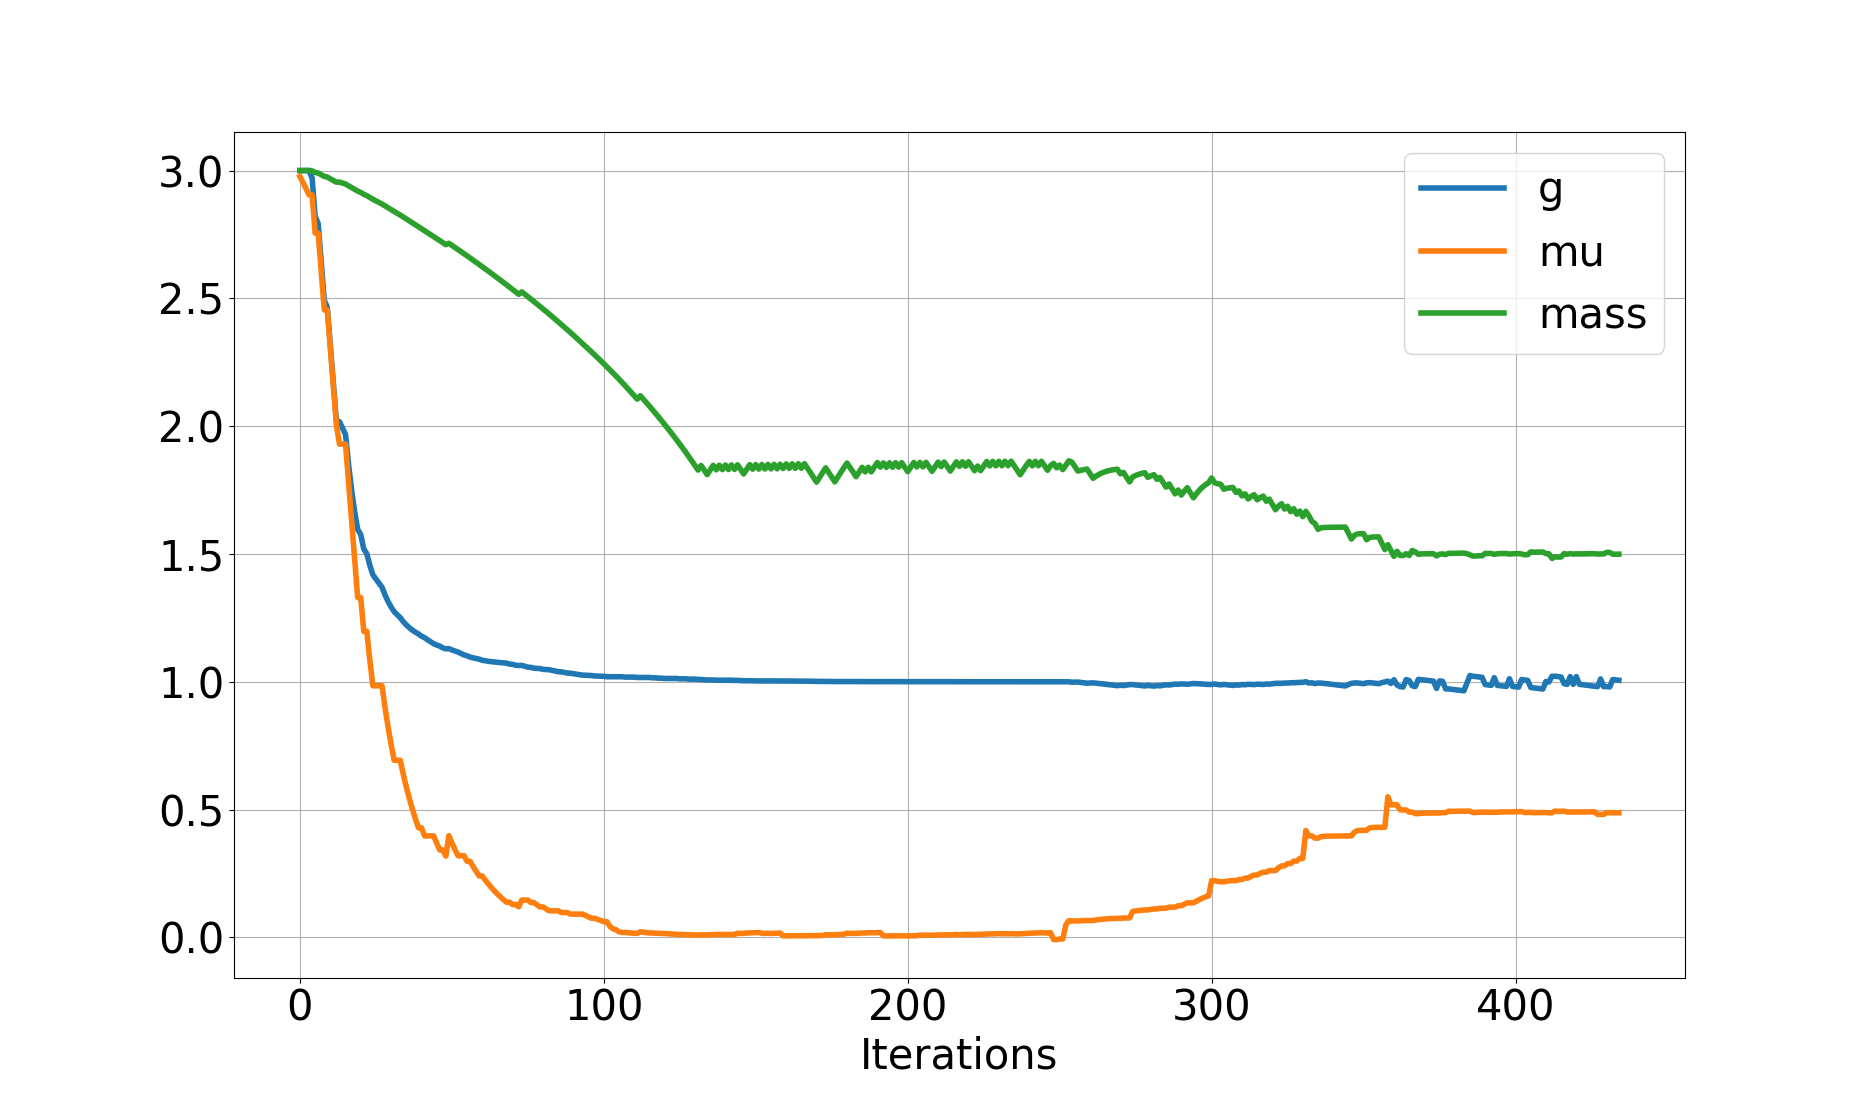
\includegraphics[width=0.8\textwidth]{three_var_learn}
              \end{figure}
             \end{block}
            
             \begin{block}{Summary}
             \textbf{Contributions}
              \begin{itemize}
                  \item Convex time-stepping contact model that addresses weaknesses of MuJoCo and Drumwright
                  \item Bilevel optimization formulation of contact dynamics learning
                  \item Expanded regions of nonzero gradients
              \end{itemize}
              \vspace{1ex}
               \textbf{Ongoing Work}             
              \begin{itemize}
                  \item Introducing learning of nonphysical quantities
                  \item Experimenting with different normal force softening methods
                  \item Testing with real Kuka arm
              \end{itemize}
            \end{block}
            
          }
          % ---------------------------------------------------------%
          % end the column
        \end{minipage}
      \end{beamercolorbox}
    \end{column}
    % ---------------------------------------------------------%
    % end the column
  \end{columns}
  
  %\begin{center} 
  %\begin{minipage}{.85 \textwidth}
  %\begin{block}{References}
  %{
  %\scriptsize
%\bibliography{library2}
%\bibliographystyle{plain}
%}
  %\end{block}   
    %\end{minipage}   
   %\end{center}
   
\end{frame}
\end{document}
